\chapter{The BONuS12 Experiment}
\label{ch:bonus}
The BONuS12 Experiment will be conducted at the Thomas Jefferson National Laboratory (JLab) in Newport News, Virginia. JLab was founded in 1984 with the intent of studying the structure of nuclear matter. The unique accelerator that was built at JLab, called the Continuous Electron Beam Accelerator Facility (CEBAF), allowed for the realization of that intent by providing for the probing of atomic nuclei at the quark level. In order to understand the BONuS12 Experiment, we must first understand CEBAF and the Hall B spectrometer that the BONuS12 RTPC will be installed in. Then we will discuss the RTPC design, components, and construction.

\begin{figure}[h!]
	\centering
	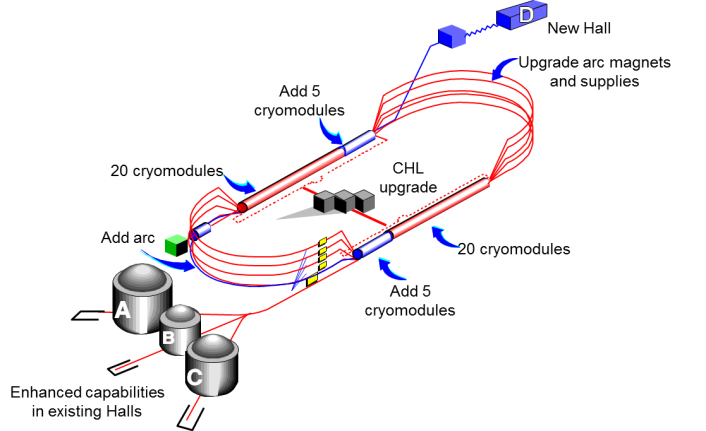
\includegraphics[width=0.8\linewidth]{figures/cebaf.png}
	\caption{CEBAF upgraded for the 12 GeV era.}
	\label{fig:cebaf}
\end{figure}

\section{Continuous Electron Beam Accelerator Facility}
The construction of the Continuous Electron Beam Accelerator Facility (CEBAF) completed in 1994. It originally consisted of two antiparallel linear accelerators (LINACs) connected by nine recirculation arcs that accelerated electrons to an energy of 6 GeV at a current of up to 300 \textmu A. In 2004, JLab began an energy upgrade that would allow CEBAF to supply electrons up to 12 GeV. The same framework used for the 6 GeV accelerator would be used for the 12 GeV era. That is, each pass around the accelerator would increase the energies, which was 1-1.2 GeV/pass during the 6 GeV era and 2.2 GeV/pass after the 12 GeV upgrade. Originally, that meant 5 passes would produce 6 GeV electrons before they were fed into the three existing experimental halls ($i.e.$ Hall A, Hall B, and Hall C). In addition to the energy upgrade that increases the energy, a new experimental hall was built ($i.e.$ Hall D). That leads to 5 passes creating an 11 GeV electron beam to Halls A, B and C. Hall D received electrons from 5.5 passes around the accelerator creating the 12 GeV electron beam energy. As Fig. \ref{fig:cebaf} shows, the upgrade consisted of addition 5 additional cryomodules, an additional recirculation arc, increased capacity of the Central Helium Liquefier (CHL), and improvements in the curving magnet.
\newline[$https://www.jlab.org/div_dept/physics_division/talks/Background/Accelerator/CEBAF_Ann_Rev_2001.pdf$]

These electrons are accelerated in CEBAF by way of the LINACs. These LINACs contain a set of superconducting Niobium accelerating cavities with a magnetic field that oscillates at a frequency of 1.5 GHz. Electrons are injected in bunches into the accelerator with an energy of 45 MeV at the same frequency as the cavities every 0.7 ns. These electrons then circulate around, increasing in energy each pass by the LINACs. Once the desired energy for a given hall is reached, the electrons are then received by the hall every 2.1 ns To go a given hall, magnetic fields inside the arcs force the electrons into specific central trajectories that guides them into that hall. The beam is considered "continuous" because of the high operating frequency at which is can operate up to its maximum capacity at 200 \textmu A.
 
\section{CEBAF Large Acceptance Spectrometer}
Once the electrons are accelerated to a desired energy, they are received by the halls, where they enter each hall's spectrometer. A spectrometer is just an instrument (or collection of instruments) that measure and analyze a range (or spectrum) of processes or reactions. Because BONuS12 will operate in Hall B, here we will focus on the components and operation of Hall B's spectrometer, called the CEBAF Large Acceptance Spectrometer at 12 GeV (or CLAS12). As the name suggests, CLAS12 is an evolution of CLAS6 (or just CLAS as it was known before talk of the energy upgrade), which was the original spectrometer built for Hall B. 

\begin{figure}[h!]
	\centering
	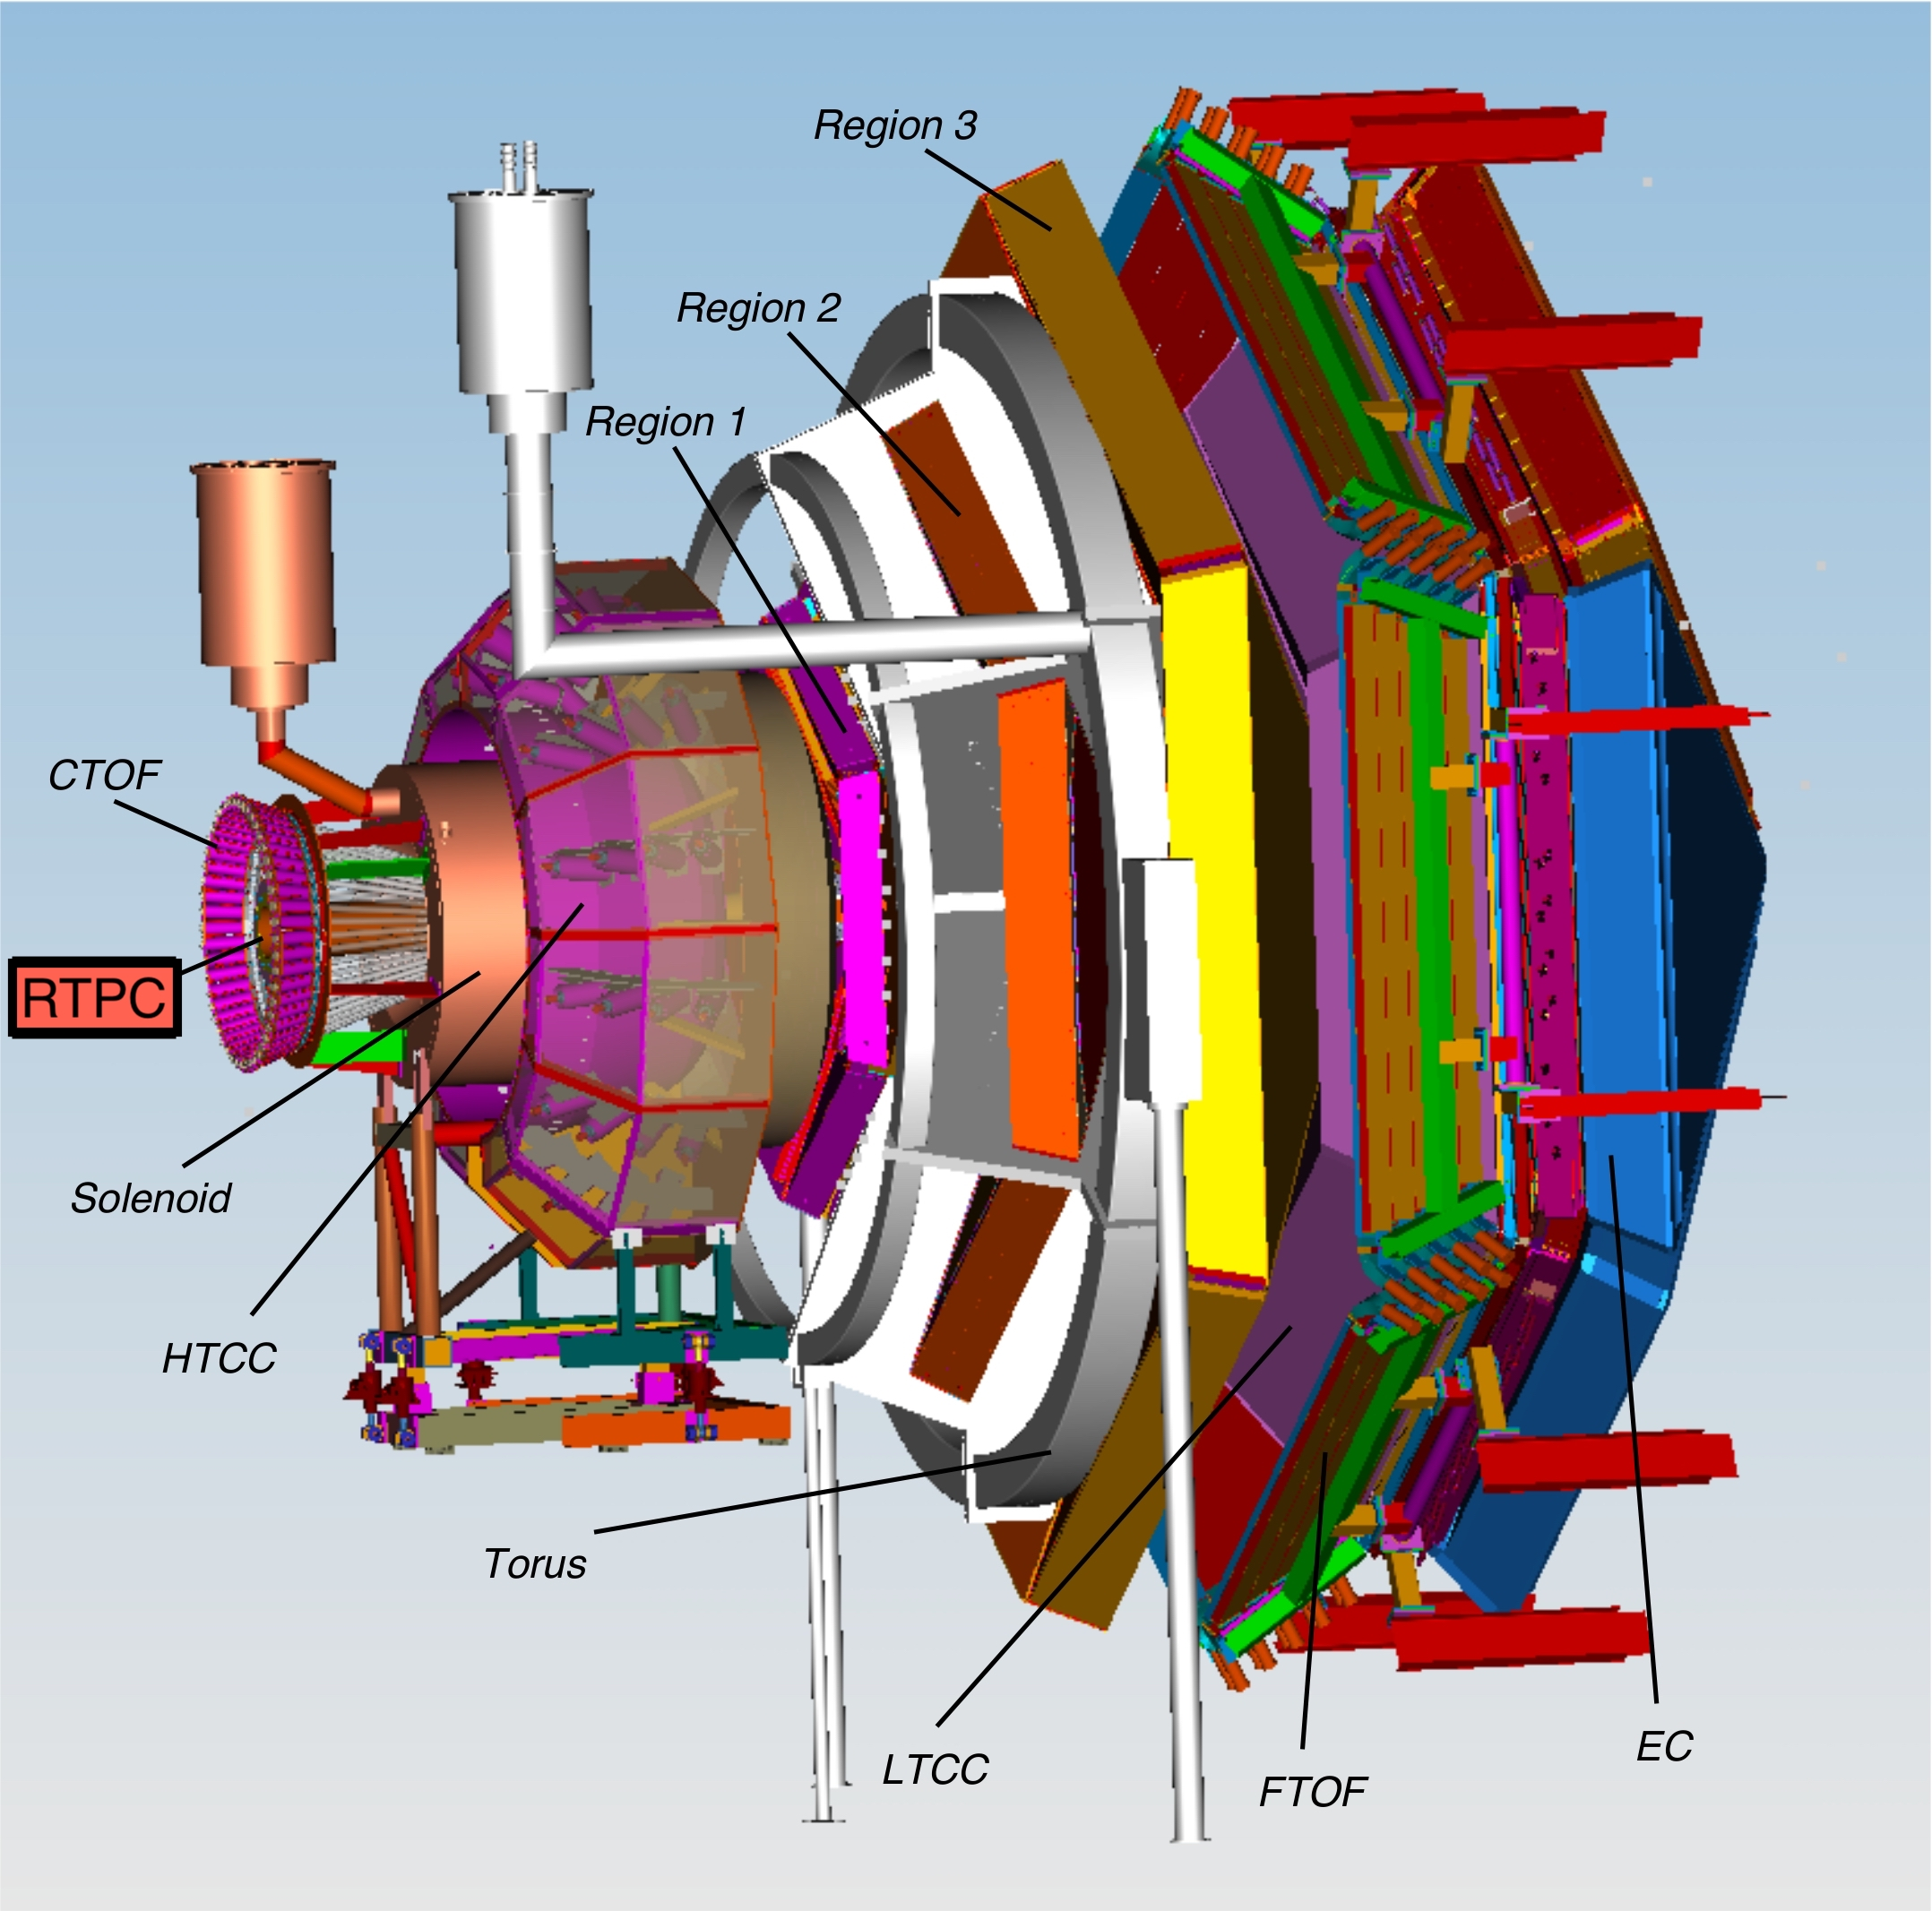
\includegraphics[width=0.8\linewidth]{figures/clas12.png}
	\caption{The CEBAF Large Acceptance Spectrometer at 12 GeV (CLAS12).}
	\label{fig:cals12}
\end{figure}

CLAS12 consists of two major groups of detectors, which together allow for detection and identification of particles over a large scattering angle, thus the "Large Acceptance" words in the name CLAS12. The Forward Detector (FD) covers scattering angles of between 5-40 degrees, and consists of a torus magnet, Cherenkov counters, a time of flight detector, drift chambers and electromagnetic calorimeter. The other group of detectors is known as the Central Detector (CD), which covers scattering angles between 40-125 degrees. The CD consists of a solenoid magnet, time of flight detector and finally, the BONuS12 RTPC. We will discuss each of these detectors, with a bit more focus on the RTPC.

\subsection{Torus Magnet}
The torus magnet is comprised of six superconducting coils arranged symmetrically around the beamline to create a azimuthally symmetric magnetic field up to 3.5 T. The coils are cooled to an operating temperature of 4.5 K by liquid helium. The shape of the coils was designed to create a field that increases near the center, which provides the desired resolution as a function of $\theta$.

The purpose of the magnetic field is to curve the tracks of charged particles without changing their azimuthal ($\phi$) angle. This curvature allows for the increased capability of particle identification. Its open structure allows for long path lengths for both charged and neutral particles, which also contributes to particle identification through time-of-flight measurements.

\subsection{Cherenkov Counters}
When a charged particle moves through a dialectric\footnote{A dialectric is any insulator that can be polarized when an electric field is applied.} with a speed greater than the phase velocity of light in that medium, electromagnetic radiation ($i.e.$ light) is emitted. This is known as Cherenkov radiation. By changing the refractive index of that medium, the threshold for emission of that light is modified. This effect allows for the distinction of particles having the same energy and momentum. By using a material with a specific refractive index, a heavier particle may not produce Cherenkov light, but a lighter particle may.

CLAS12 contains two detectors that exploit this Cherenkov effect. The High Threshold Cherenkov Counter (HTCC) is between the solenoid and the first region of the Drift Chambers. It discriminates electrons and pions by being filled with CO$_2$. This gas has an index of refraction $n=1.00041$, which forces pion above 4.6 GeV to produce light. If the particle has an energy below this threshold and it produces light, it is an electron. The other Cherenkov detector is the Low Threshold Cerenkov Counter (LTCC), which sits between Region 3 of the Drift Chambers and the Forward Time of Flight detector. It is filled with C$_4$F$_12$, which allows for the discrimination of pions and kaons at the 2.6 GeV where only pions produce Cherenkov light.

\subsection{Drift Chambers}
There are three regions of Drift Chambers (DC) that collectively allow for the reconstruction of charged particle trajectories. The first region is located in front of the Torus Magnet out the reach of the field. Region 2 is between the coils in the high field region. The third region is after the Torus, but feels a small magnetic field from the coils. Each region is made of six triangular sectors, which are made of small wires and filled with a gas mixture that exploits the process of ionization.

Within the sectors of the DC there are hundreds of wires, half of which are positive and the other half negative. When a charged particle travels through the gas mixture (90$\%$ Argon 10$\%$ CO$_2$ for the case of the CLAS12 DC), it knocks off electrons from the gas molecules as it passes. This process is known as $ionization$. In the DC, these ionization electrons that are created as charged particles pass through are accelerated to the nearest positive wire from the electric field created by the negative-positive wire pairs. The ion created is accelerated toward the nearest negative wire by the same electric field.

Using the signals created by the electron-ion pairs as the charged particle travels through the regions of the DC allow for the reconstruction of that particle's path. This information lends itself to the reconstruction of the particle momentum as well as its vertex ($i.e.$ where the particle collision occurred).
\subsection{Forward Time of Flight}
\subsection{Electromagnetic Calorimeter}
\subsection{Central Time of Flight}
\subsection{Solenoid Magnet}

\section{BONuS12 RTPC}
\subsection{Target}
\subsection{Cathode and Ground Foil}
\subsection{Sensitive Region}
\subsection{Gaseous Electron Multiplier Foils}
\subsection{Readout Pad-Board}
\subsection{Translation Boards and Electronics}
\subsection{Construction and Integration}

\section{Drift-Gas Monitoring System}
\label{sec:dms}
\subsection{Purpose}
\subsection{Electric Field}
\subsection{Design}
\subsection{Construction and Testing}
\subsection{Integration}

